\documentclass[pdftex,sn-mathphys-num]{sn-jnl}

\usepackage{graphicx}
\usepackage{amsmath,amssymb,amsfonts}
\usepackage{booktabs}
\usepackage{array}
\usepackage{tabularx}
\usepackage{longtable}
\usepackage{multirow}
\usepackage{makecell}
\usepackage{ragged2e}
\usepackage{url}
\usepackage{microtype}
\usepackage{caption}
\usepackage{placeins}
\usepackage{enumitem}
\usepackage{algorithm}
\usepackage{algpseudocode}
\usepackage{xcolor}
\usepackage{needspace}

\raggedbottom
\setlength{\LTpre}{6pt}
\setlength{\LTpost}{4pt}
\setlength{\LTleft}{0pt}
\setlength{\LTright}{0pt}
\setlength{\tabcolsep}{2.5pt}
\renewcommand{\arraystretch}{0.92}

\begin{document}

\title[Integrated Indian trade analytics]{A Comprehensive Integrated Framework for International Demand and Supply Analytics and Forecasting: An Indian Commodity Context}

\author[1]{\fnm{Aaradhy} \sur{Pandey}}
\author*[1]{\fnm{Tusar Kanti} \sur{Mishra}}\email{tusar.mishra@manipal.edu}

\affil[1]{\orgdiv{Manipal Institute of Technology Bengaluru}, \orgname{Manipal Academy of Higher Education}, \orgaddress{\city{Manipal}, \country{India}}
}
\abstract{The framework examines international demand-supply forecasting in the Indian context, giving attention to the events where fluctuations occured in the market conditions. It combines Particle Swarm Optimization (PSO), monthly Local Interpretable Model-agnostic Explanations (LIME), and yearly SHapley Additive exPlanations (SHAP) to support both forecasting and the interpretation of its results.It uses a dataset containing 60 monthly observations from January 2021 to December 2025, covering six sectors of Indian trade.Crude oil, cotton, and electronic circuits are treated as international-demand tasks because import quantity is the selected target, whereas rice, packed medicine, and spices are treated as international-supply tasks because export quantity is the selected target. Every month is retained and classified as SURGE, DROP, or REGULAR by converting the month-on-month target change into a sample-standard-deviation z-score and applying the fixed threshold $|z|=1.5$ inherited from the specified event-classification rule. The PSO formulation follows the required full-vector representation: each particle contains one continuous weight for every predictor and the swarm iteratively updates particles toward personal best and global best states under a minimum-error objective. Explainable artificial intelligence (XAI) is then used at two temporal resolutions. LIME produces a local explanation for each month, while SHAP aggregates additive feature contributions by calendar year. Because raw LIME coefficients and PSO weights have different scales, their absolute local contribution magnitudes are normalised within each month to a common 0--100\% share. The dominant LIME feature is compared with the PSO-induced local share of that same feature and a difference above 10 percentage points is marked as an outlier.Out of a total of 360 monthly observations across all six sectors, 26 months are classified as SURGE, 18 as DROP, and the remaining 316 as REGULAR. The difference between LIME and PSO on the performance comparison scale was, on average, 2.16 percentage points. However, one non-fluctuation month had a difference greater than 10 percentage points, so that month is considered an outlier. The framework connects fluctuation detection, PSO optimisation, LIME explanation, and yearly SHAP attribution.
}

\keywords{Indian international trade, demand analytics, supply analytics, Particle Swarm Optimization, LIME, SHAP, explainable artificial intelligence, fluctuation events, commodity analytics}

\maketitle

\section{Introduction}
International trade is rarely shaped by only one factor. Some of the factors that actively influence trade include domestic production and consumption, inventory levels, prices, exchange rates, investment, and changes in external markets. Therefore, a fluctuation in a particular month can be influenced by one or more factors acting simultaneously, sometimes in different directions. From this, two broad questions arise. First, to identify whether the monthly data differs significantly from the historical behaviour of the same series. Second, if a significant difference is observed, why does the analytical model assign greater weight to certain predictors for that particular month of fluctuation
.It is strongly relevant to Indian trade, as different sectors have distinct trade trajectories for imports and exports because some series reflect strong domestic demand, some reflect exportable production and stock availability, and others are sensitive to international prices and exchange-rate conditions. Methods using machine learning are increasingly deployed to understand non-linear relationships in international trade and combine structural and temporal information to achieve real-time nowcasting.
 \cite{josic2022,chinn2023,yang2023}.However, the influence of a variable during a particular month cannot be pointed out by the model. Explainable Artificial Intelligence (XAI) bridges this gap by providing explanations for the contribution of model inputs to individual predictions. The XAI
literature differentiates local and global explanation, model-agnostic and model-specific
approaches, and qualities such as faithfulness, stability, transparency, and usefulness\cite{guidotti2018,arrieta2020,schwalbe2024,mersha2024,abusitta2024,longo2024}. In this study, we use XAI as a part of the analysis framework: LIME explains the model's prediction for a particular month, and SHAP summarises the changes in variables across the year rather than just focusing on one month.

This study is built from the dataset of six different sectors covering the period from January 2021 to December 2025. Crude oil, cotton, and electronic circuits are selected as import quantities. Rice, packed medicine, and spices are selected as export quantities. This mapping is kept fixed throughout the analysis. The workbook provides common trade, balance, price, exchange-rate, and investment variables, allowing the six tasks to be examined within one methodological architecture while preserving their different meanings. The monthly trade data is consistent with TRADESTAT, where the Government of India's monthly foreign-trade reports are available and arranged commodity-wise.\cite{tradestat}. Event classification rules are applied to each month's observations for the initial analysis. The difference in the target value between two consecutive months is converted into a z-score using the sample standard deviation. A fixed threshold of 1.5 is then applied to classify each month as SURGE, DROP, or REGULAR, depending on the size and direction of the change. No observation is removed because of its event status. By doing this, we get a complete calendar in which fluctuation events are identified independently of the later XAI calculations. Recent research in India has explored how different features behave in monthly trade forecasting. Similarly, international research suggests that machine-learning models can capture nonlinear relationships between trade and economic variables.\cite{balasubramanian2026,josic2022,yang2023,chinn2023}. The present study extends this application space by connecting event detection to a globally optimised feature-weight structure and then testing how closely the local explanation for each month follows that global weighting pattern.

XAI is particularly relevant because the same global model can behave differently across neighbouring months. LIME constructs a locally weighted surrogate around a selected observation and uses the surrogate coefficients to describe the local contribution of each feature \cite{ribeiro2016}. SHAP provides an additive Shapley-based attribution framework that can be aggregated across observations \cite{lundberg2017}. These approaches are complementary rather than interchangeable. A local LIME contribution answers the question ``what drove this month's model response?'', whereas an annual SHAP profile asks ``which variables contributed most when the month's explanations are considered across this year?'' Research on dependent features and causal interpretation also shows why attribution should not automatically be read as a structural economic effect \cite{aas2021,janzing2020}. Temporal XAI research further suggests that the time-local behaviour of explanations should be retained rather than reduced to one static feature ranking \cite{canti2024,vanzy2024,hertel2026}. PSO supplies a third perspective. The original algorithm searches a population of candidate solutions using inertia and attraction toward personal and global best positions \cite{kennedy1995,shi1998,clerc2002,poli2007}, while later studies adapt PSO through grouped variables, historical-success guidance, adaptive pyramid search, and ecology-inspired feature selection \cite{gao2024,gupta2024,jin2024,pepspso2025}. In this study, however, PSO is not added as a generic optimiser. Each particle is explicitly constructed from the predictor columns of one trade sheet, every predictor receives a continuous weight, the swarm is calibrated on the first 48 months, and the final global-best vector is carried into the monthly explanation stage. This makes the optimisation layer directly interpretable in terms of the actual variables in the dataset.

The contribution is the integration of four linked functions into one reproducible event-aware workflow. The event layer labels every month as SURGE, DROP, or REGULAR; PSO searches a complete feature-weight vector for each sector-task; LIME explains the local response of each month; and SHAP summarises feature contributions by year. Because LIME coefficients and PSO weights are not directly comparable, both are converted into monthly percentage-contribution shares. The dominant LIME feature is paired with the PSO-induced share of the same feature, and their absolute difference in percentage points is used as the agreement statistic. A difference above 10 percentage points is an explanation outlier, independently of the trade-event label. The analysis focuses on identifying distinctive months, examining the feature-weight vector having a specific weight for a feature that PSO converges to and finding out which variable has the highest influence on monthly predictions. It compares the performance of LIME and PSO algorithm and uses yearly SHAP results to examine how feature contributions change over time. The overall aim is to develop a transparent approach to analysing fluctuations in Indian trade, rather than to claim that the model is universally superior or that the identified relationships establish causation.

\section{Background and Related Work}
Research relevant to the framework lies at the intersection of optimisation, explainable artificial intelligence, and international-trade analytics. PSO is attractive as a global weighting mechanism because it searches a population of candidate vectors rather than relying on a single local update trajectory. The foundational algorithm established the inertia, personal-best, and global-best structure, while later work formalised convergence behaviour and demonstrated how PSO can be adapted for feature selection and feature weighting \cite{kennedy1995,shi1998,clerc2002,poli2007}. More recent work introduces information-gain-based feature grouping, historical-success guidance, adaptive pyramid search, and ecology-inspired feature-selection strategies \cite{gao2024,gupta2024,jin2024,pepspso2025}. These developments motivate the use of a population-based optimiser while leaving room for application-specific formulation. On the XAI side, LIME established a model-agnostic local surrogate approach \cite{ribeiro2016}, while SHAP introduced a Shapley-based additive framework for prediction explanation \cite{lundberg2017}. Subsequent work has examined feature dependence, causal interpretation, and the broader conditions under which an explanation can be considered useful or faithful \cite{aas2021,janzing2020,guidotti2018,schwalbe2024,mersha2024,abusitta2024,longo2024}. Recent temporal-XAI studies indicate that explanation methods should preserve the time-local structure of a model rather than collapsing every observation into one static ranking \cite{canti2024,vanzy2024,hertel2026}. These strands jointly support the architecture used here: optimisation defines a global feature-weight structure, LIME explains individual monthly responses, and SHAP provides a calendar-year attribution profile.

International-trade forecasting research supplies the application context. Machine-learning approaches have been used to predict international trade flows, to nowcast world trade from high-frequency information, and to combine economic and trade variables in nonlinear prediction systems \cite{josic2022,chinn2023,yang2023}. Indian research has recently examined monthly trade forecasting and feature-learning behaviour \cite{balasubramanian2026}. The Government of India's TRADESTAT system provides a corresponding data infrastructure for monthly import and export analysis \cite{tradestat}. What is less directly addressed by these strands is the specific combination studied here: an explicit monthly event calendar, a full-vector PSO optimisation tied to the supplied trade columns, a monthwise LIME layer, a yearly SHAP layer, and a common-scale LIME--PSO agreement diagnostic. The contribution is therefore best understood as an integrated methodological application rather than a claim that PSO, LIME, or SHAP is itself new. The research also deliberately keeps attribution separate from causality because several supplied variables can be mechanically or economically related, including trade quantity and trade value, stock variables, and price variables. This interpretive caution follows established XAI work that distinguishes predictive relevance from structural or causal effect \cite{janzing2020,longo2024,rudin2019}.

\section{Data and Integrated Methodology}
The supplied workbook contains six sector sheets with 60 monthly observations from January 2021 through December 2025 and a common family of trade, balance, price, exchange-rate, and investment variables. Crude oil, cotton, and electronic circuits are mapped to import quantity and interpreted as international-demand tasks; rice, packed medicine, and spices are mapped to export quantity and interpreted as international-supply tasks. For an import task, the corresponding import-value column is excluded from the predictor vector; for an export task, the corresponding export-value column is excluded. Year and Month are used only for temporal ordering and event labelling, not as model predictors. The remaining variables form the sector-specific feature space. Predictor means and standard deviations are calculated from the first 48 observations, January 2021 through December 2024, and the same calibration statistics are used to standardise all 60 observations. The target is standardised for the PSO fitting objective. This fixed calibration boundary is chosen so that the model configuration is established before the 2025 monthly explanations are interpreted. The six sector-task series therefore remain comparable at the workflow level without pretending that they represent the same economic mechanism.

\begin{figure}[t]
\centering
% \includegraphics[width=0.96\linewidth]{figures/framework1.pdf}
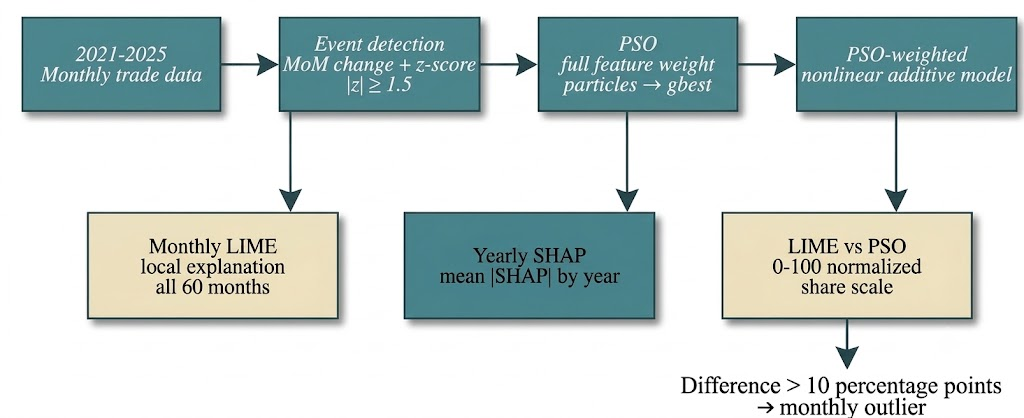
\includegraphics[width=0.96\linewidth]{frame1.jpg}
\caption{Architecture of the proposed Indian trade XAI framework. The workflow maps the six sectors to import-demand or export-supply tasks, labels every month using the 1.5 z-score event rule, optimises a full feature-weight vector with PSO, produces monthwise LIME and yearly SHAP explanations, and compares LIME with PSO on a common local-contribution scale.}
\label{fig:architecture}
\end{figure}

The event mechanism follows the supplied specified event-classification rule. For target quantity $Y_t$, the month-on-month relative change is
\begin{equation}
\Delta_t=\frac{Y_t-Y_{t-1}}{Y_{t-1}}.
\end{equation}
The first month has no predecessor and is therefore labelled REGULAR. For the remaining months, the sample mean $\bar{\Delta}$ and sample standard deviation $s_\Delta$ of the monthly changes are used to calculate
\begin{equation}
z_t=\frac{\Delta_t-\bar{\Delta}}{s_\Delta}.
\end{equation}
The fixed classification is
\begin{equation}
\mathrm{Event}_t=\begin{cases}
\mathrm{SURGE}, & z_t\geq1.5,\\
\mathrm{DROP}, & z_t\leq-1.5,\\
\mathrm{REGULAR}, & -1.5<z_t<1.5.
\end{cases}
\end{equation}
No month is removed because of this label. Applying the rule to the six sector-task series gives 26 SURGE, 18 DROP, and 316 REGULAR observations. The event label is intentionally independent of the later LIME--PSO outlier label: the former identifies an unusual movement in the target series, while the latter identifies a large local-versus-global explanation difference.

For $d$ eligible predictors, particle $k$ at iteration $r$ is the full feature-weight vector
$W_k^{r}=[w_{k1}^{r},\ldots,w_{kd}^{r}]$. After calibration on the first $T=48$ months, the response surface is
$g(x)=0.2x+0.8\tanh(x)$ and
$\hat y_{k,t}=\sum_{i=1}^{d}w_{ki}^{r}g(x_{i,t})$.
The objective is the 48-month mean squared fitting loss with a small $\ell_2$ penalty. The swarm update is
\begin{equation}
V_k^{r+1}=\omega_rV_k^r+c_1r_{1}(P_k^r-W_k^r)+c_2r_{2}(G^r-W_k^r),
\end{equation}
\begin{equation}
W_k^{r+1}=\operatorname{clip}(W_k^r+V_k^{r+1},-2,2).
\end{equation}
Here, $P_k$ and $G$ are the particle best and swarm best, $\omega_r$ decreases from 0.9 to 0.5, and $c_1=c_2=1.6$. We use $N=80$ particles and $R=250$ iterations; the final $G$ is the sector-specific global weight vector used in every subsequent monthly explanation.

\begin{algorithm}[t]
\caption{Dataset-specific PSO algorithm}
\label{alg:pso}
\begin{algorithmic}[1]
\Require Sector sheet $S$, target $Y$, predictors $X$, $T=48$, $N=80$, $R=250$.
\State $X\leftarrow$ eligible trade predictors; remove $Y$, its matching value column, Year, and Month.
\State Standardise $X$ and $Y$ with means and standard deviations computed on $t\leq T$.
\State Initialise $W_k^0\in[-1.5,1.5]^d$ and $V_k^0\in[-0.2,0.2]^d$, $k=1,\ldots,N$.
\State Evaluate $F(W_k^0)$; set $P_k=W_k^0$ and $G=\arg\min_k F(P_k)$.
\For{$r=0,\ldots,R-1$}
  \State $\omega_r=0.9-0.4r/(R-1)$.
  \State Update $V_k$ and $W_k$ with $P_k$, $G$, $c_1=c_2=1.6$; clip $W_k$ to $[-2,2]$.
  \State Recompute $F(W_k)$; update $P_k$ and $G$ whenever $F$ decreases.
\EndFor
\State Return sector $gbest=G$; reuse $G$ for all monthly LIME and yearly SHAP calculations.
\end{algorithmic}
\end{algorithm}

The comparison layer converts the two explanation systems to a common monthly scale. If $c_{i,t}$ denotes the LIME surrogate coefficient for feature $i$ in month $t$, its local contribution share is
\begin{equation}
L_{i,t}=100\times\frac{|c_{i,t}x_{i,t}|}{\sum_j|c_{j,t}x_{j,t}|}.
\end{equation}
For the final PSO vector, the corresponding local contribution is $q_{i,t}=|w_i^*g(x_{i,t})|$ and the normalised share is
\begin{equation}
Q_{i,t}=100\times\frac{q_{i,t}}{\sum_jq_{j,t}}.
\end{equation}
Both therefore sum to 100\% within each month. The dominant LIME variable is $i^*(t)=\arg\max_i L_{i,t}$, and the monthwise agreement difference is
\begin{equation}
D_t=|L_{i^*(t),t}-Q_{i^*(t),t}|.
\end{equation}
The result is expressed in percentage points. A month is labelled OUTLIER only when $D_t>10$. This threshold serves as an explanation for the considerable difference between local and global explanations. It does not classify another type of trade fluctuation.


3,000 perturbed samples are generated for the monthly LIME analysis around each observation. Samples that are closer to the original observation are given greater weight in the ridge surrogate that is fitted to the PSO response surface. In order to compare the dominant factor month by month, the local contributions are normalised to the common share scale. For the yearly SHAP analysis, the response surface is additive in the transformed features, which allows each feature's contribution to be calculated directly.

\begin{equation}
\phi_{i,t}=w_i^*\left[g(x_{i,t})-E_{\mathrm{cal}}g(X_i)\right]
\end{equation}

These contributions are then categorized based on the calendar year and their absolute values. The annual contributions are transformed to a scale of 100\% within each sector-year, which makes it convenient to compare the importance of different features relatively. The resulting analytical design therefore has a clear temporal separation: the event layer labels every month, LIME explains the local month, PSO supplies the global weight structure, and SHAP summarises the yearly contribution profile.

\section{Results and Interpretation}
The exact event classification preserves all 360 sector-month observations and yields 26 SURGE, 18 DROP, and 316 REGULAR months. Crude oil contains five SURGE and three DROP observations; cotton contains four and three; electronic circuits contains three and three; rice contains five and three; packed medicine contains four and one; and spices contains five and five. The crude-oil event calendar reproduces the specified event-classification rule events: August 2021 and September 2021 are DROP, January 2022 is SURGE, July 2022 is DROP, January 2023 is SURGE, November 2023 is SURGE, January 2024 is SURGE, and December 2024 is SURGE. The corresponding events for the remaining five tasks are generated by the same unmodified $|z|\geq1.5$ rule. Figure~\ref{fig:calendar} visualises when SURGE and DROP observations occur across sectors, while Table~\ref{tab:events} condenses the same event structure into sector totals and adds the explanation-agreement statistics. Together they show that fluctuation detection and explanation agreement are separate analytical layers: the event labels are generated first and are never influenced by the LIME--PSO result.

\begin{figure}[!ht]
\centering
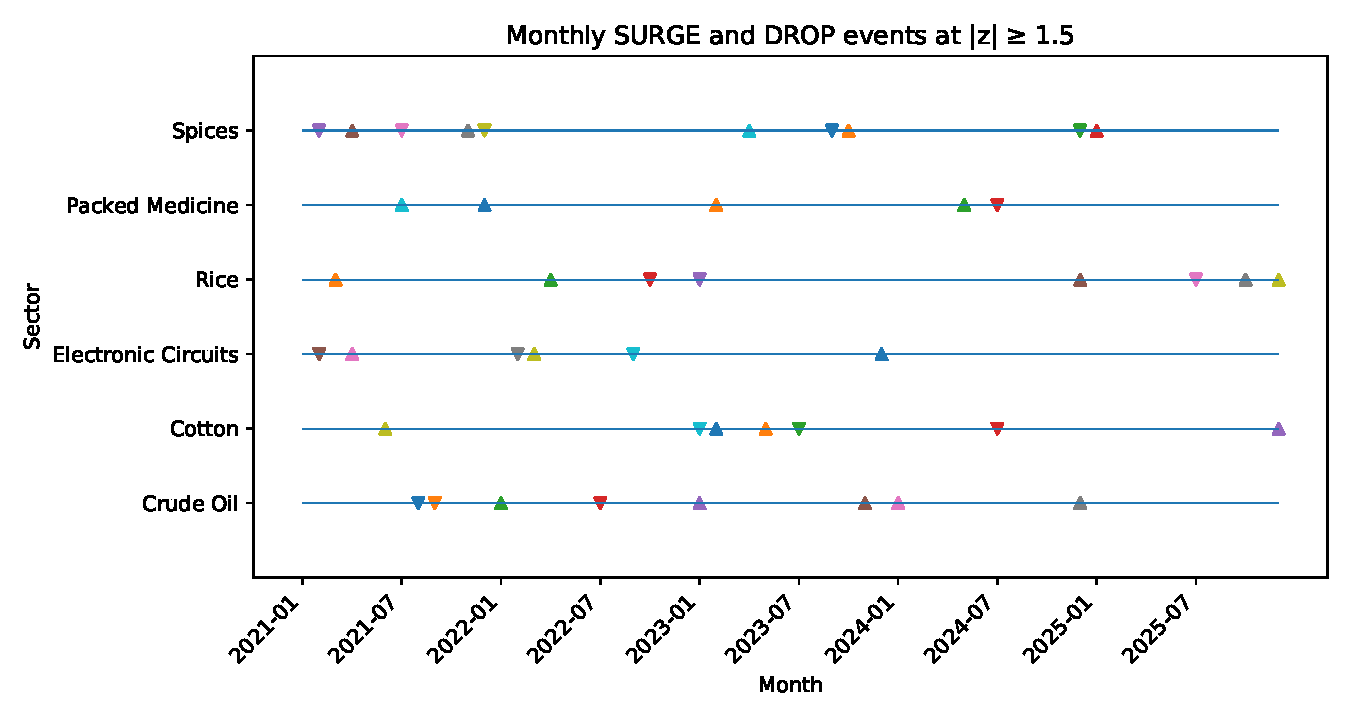
\includegraphics[width=\textwidth]{figures/event_calendar.pdf}
\caption{Monthly SURGE and DROP events across the six sector-task series using the fixed $|z|\geq1.5$ rule. REGULAR observations remain in the complete monthwise tables.}
\label{fig:calendar}
\end{figure}

\begin{table}[!ht]
\caption{Event counts and LIME--PSO agreement by sector. $D_t$ is measured in percentage points on the common local-contribution-share scale.}
\label{tab:events}
\centering
\small
\begin{tabular}{lrrrrrr}
\toprule
Sector & SURGE & DROP & REGULAR & Mean $D_t$ & Max $D_t$ & Outliers\\
\midrule
Crude oil & 5 & 3 & 52 & 3.90 & 12.16 & 1\\
Cotton & 4 & 3 & 53 & 1.61 & 5.95 & 0\\
Electronic circuits & 3 & 3 & 54 & 1.65 & 5.89 & 0\\
Rice & 5 & 3 & 52 & 1.96 & 4.39 & 0\\
Packed medicine & 4 & 1 & 55 & 1.76 & 4.34 & 0\\
Spices & 5 & 5 & 50 & 2.09 & 5.87 & 0\\
\midrule
All sectors & 26 & 18 & 316 & 2.16 & 12.16 & 1\\
\end{tabular}
\end{table}

Table~\ref{tab:events} shows that most sector-months are REGULAR and that the single explanation outlier is concentrated in crude oil; the maximum gap for the other sectors remains below the 10-point threshold.

The PSO swarm converges from complete feature-weight arrays to one final $gbest$ vector for each sector-task. The largest normalised $gbest$ shares are domestic consumption for crude oil (62.5\%) and electronic circuits (40.3\%), domestic production for cotton (16.3\%), rice (19.0\%), and spices (24.6\%), and opening stock for packed medicine (21.9\%). These are model weights within the defined response surface rather than causal elasticities. Figure~\ref{fig:pso} presents the convergence histories and makes the optimisation behaviour visible across all six tasks. The monthwise LIME--PSO tables then use the same sector-specific $gbest$ vectors for every month, so the comparison is between a fixed global weighting structure and month-specific local explanations rather than between separately re-optimised models.

\begin{figure}[!ht]
\centering
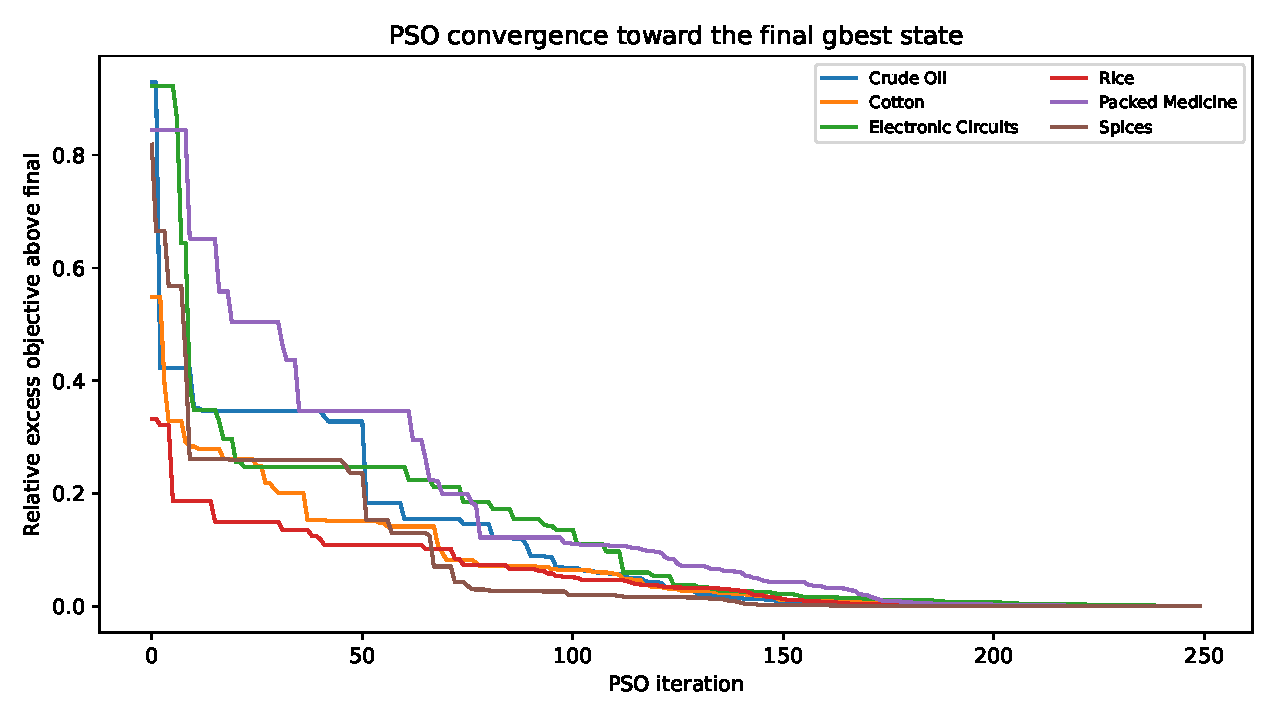
\includegraphics[width=0.96\linewidth]{figures/pso_convergence.pdf}
\caption{PSO convergence toward the final global-best objective state for the six sector-task series.}
\label{fig:pso}
\end{figure}

\FloatBarrier
\vspace{4pt}

% Compact keys used throughout the monthwise LIME--PSO tables.
{\scriptsize\noindent\textbf{Feature names:} Prod = Domestic Production; Cons = Domestic Consumption; OpenStk = Opening Stock; CloseStk = Closing Stock; StockChg = Stock Change; WPI = Domestic Wholesale Price; GlobalP = Global Benchmark Price; FX = Exchange Rate; Capex = Sector Investment; ImpQ = Import Quantity; ImpV = Import Value; ExpQ = Export Quantity; ExpV = Export Value.}\par\vspace{1pt}
{\tiny\noindent\textbf{Column key:} E = Event; F = Feature; L = LIME share (\%); P = PSO share (\%); $\Delta$ = LIME--PSO difference (percentage points).}\par\vspace{1pt}
% Two-page portrait monthwise LIME--PSO comparison tables (native LaTeX longtable).
% longtable keeps caption attached to the table on its own page and handles page breaks cleanly.
\begingroup
\setlength{\tabcolsep}{3pt}
\renewcommand{\arraystretch}{1.08}
\scriptsize
\begin{longtable}{%
  >{\raggedright}p{1.10cm}%   Mo.
  >{\raggedright}p{4.05cm}%   Crude oil
  >{\raggedright}p{4.05cm}%   Cotton
  >{\raggedright}p{4.05cm}%   Electronic circuits
}
\caption{Monthwise LIME--PSO comparison for international-demand tasks (imports), January 2021--December 2025.
Each cell reports: \textbf{E} (event: S=surge, D=drop, R=regular) | \textbf{F} (dominant feature) | \textbf{L} (LIME share, \%) | \textbf{P} (PSO share, \%) | $\boldsymbol{\Delta}$ (difference, percentage points). Asterisk (*) marks $\Delta>10$\,pp.}
\label{tab:limepso_demand}\\
\toprule
\textbf{Mo.} &
\parbox[c]{4.00cm}{\centering\small\textbf{Crude oil}\\[1pt]\textbf{E\,|\,F\,|\,L\,|\,P\,|\,$\Delta$}} &
\parbox[c]{4.00cm}{\centering\small\textbf{Cotton}\\[1pt]\textbf{E\,|\,F\,|\,L\,|\,P\,|\,$\Delta$}} &
\parbox[c]{4.00cm}{\centering\small\textbf{Electronic circuits}\\[1pt]\textbf{E\,|\,F\,|\,L\,|\,P\,|\,$\Delta$}}\\
\midrule
\endfirsthead
\multicolumn{4}{l}{\small\textit{(Table~\ref{tab:limepso_demand} continued)}}\\[2pt]
\toprule
\textbf{Mo.} &
\parbox[c]{4.00cm}{\centering\small\textbf{Crude oil}\\[1pt]\textbf{E\,|\,F\,|\,L\,|\,P\,|\,$\Delta$}} &
\parbox[c]{4.00cm}{\centering\small\textbf{Cotton}\\[1pt]\textbf{E\,|\,F\,|\,L\,|\,P\,|\,$\Delta$}} &
\parbox[c]{4.00cm}{\centering\small\textbf{Electronic circuits}\\[1pt]\textbf{E\,|\,F\,|\,L\,|\,P\,|\,$\Delta$}}\\
\midrule
\endhead
\midrule
\multicolumn{4}{r}{\small\textit{Continued on next page}}\\
\endfoot
\bottomrule
\endlastfoot
\enlargethispage{2\baselineskip}%
Jan-21 & R-Cons\,|\,63.9\,|\,63.7\,|\,0.2 & R-WPI\,|\,17.6\,|\,19.1\,|\,1.5 & R-Cons\,|\,41.2\,|\,40.1\,|\,1.1 \\
Feb-21 & R-Cons\,|\,60.1\,|\,52.3\,|\,7.8 & R-dStk\,|\,19.5\,|\,20.3\,|\,0.7 & D-Cons\,|\,41.2\,|\,45.4\,|\,4.2 \\
Mar-21 & R-Cons\,|\,42.3\,|\,34.2\,|\,8.1 & R-WPI\,|\,16.9\,|\,15.4\,|\,1.5 & R-Cons\,|\,40.0\,|\,42.9\,|\,2.9 \\
Apr-21 & R-dStk\,|\,25.8\,|\,31.5\,|\,5.6 & R-dStk\,|\,18.4\,|\,16.5\,|\,1.9 & S-Cons\,|\,41.3\,|\,38.7\,|\,2.6 \\
May-21 & R-Capex\,|\,25.9\,|\,28.9\,|\,2.9 & R-Capex\,|\,22.0\,|\,28.0\,|\,5.9 & R-Cons\,|\,41.2\,|\,39.6\,|\,1.6 \\
Jun-21 & R-Cons\,|\,61.7\,|\,55.0\,|\,6.7 & S-Prod\,|\,21.9\,|\,21.9\,|\,0.0 & R-Cons\,|\,41.8\,|\,42.5\,|\,0.7 \\
Jul-21 & R-Cons\,|\,38.7\,|\,31.4\,|\,7.4 & R-Prod\,|\,24.5\,|\,24.3\,|\,0.2 & R-Cons\,|\,40.7\,|\,41.1\,|\,0.4 \\
Aug-21 & D-Cons\,|\,62.5\,|\,60.5\,|\,2.0 & R-Prod\,|\,25.1\,|\,25.0\,|\,0.1 & R-Cons\,|\,40.4\,|\,40.4\,|\,0.0 \\
Sep-21 & D-Cons\,|\,65.1\,|\,70.1\,|\,5.0 & R-Prod\,|\,18.3\,|\,18.7\,|\,0.4 & R-Cons\,|\,40.7\,|\,42.9\,|\,2.2 \\
Oct-21 & R-Cons\,|\,67.3\,|\,74.8\,|\,7.5 & R-dStk\,|\,16.9\,|\,15.0\,|\,1.9 & R-Cons\,|\,43.4\,|\,46.3\,|\,3.0 \\
Nov-21 & R-Cons\,|\,65.0\,|\,71.1\,|\,6.1 & R-Prod\,|\,17.2\,|\,17.0\,|\,0.2 & R-Cons\,|\,41.0\,|\,41.1\,|\,0.1 \\
Dec-21 & R-Cons\,|\,63.3\,|\,63.4\,|\,0.1 & R-WPI\,|\,16.5\,|\,15.9\,|\,0.6 & R-Cons\,|\,43.6\,|\,45.6\,|\,2.0 \\
Jan-22 & S-Cons\,|\,62.2\,|\,59.8\,|\,2.4 & R-WPI\,|\,17.0\,|\,17.9\,|\,0.9 & R-Cons\,|\,35.1\,|\,32.6\,|\,2.5 \\
Feb-22 & R-dStk\,|\,34.0\,|\,38.0\,|\,4.0 & R-WPI\,|\,17.6\,|\,19.9\,|\,2.4 & D-Cons\,|\,42.6\,|\,43.6\,|\,1.0 \\
Mar-22 & R-Cons\,|\,51.0\,|\,44.1\,|\,6.9 & R-WPI\,|\,18.9\,|\,20.6\,|\,1.7 & S-Cons\,|\,30.5\,|\,29.1\,|\,1.4 \\
Apr-22 & R-Cons\,|\,62.2\,|\,60.6\,|\,1.6 & R-WPI\,|\,22.2\,|\,27.9\,|\,5.6 & R-Cons\,|\,34.0\,|\,32.2\,|\,1.8 \\
May-22 & R-dStk\,|\,39.2\,|\,40.3\,|\,1.1 & R-WPI\,|\,21.7\,|\,26.4\,|\,4.7 & R-Cons\,|\,31.9\,|\,29.8\,|\,2.1 \\
Jun-22 & R-dStk\,|\,41.4\,|\,38.7\,|\,2.7 & R-dStk\,|\,21.9\,|\,23.0\,|\,1.1 & R-ExpV\,|\,31.8\,|\,32.4\,|\,0.6 \\
Jul-22 & D-Cons\,|\,56.8\,|\,53.7\,|\,3.1 & R-dStk\,|\,20.8\,|\,23.0\,|\,2.3 & R-ExpQ\,|\,23.6\,|\,22.8\,|\,0.8 \\
Aug-22 & R-Cons\,|\,73.0\,|\,77.1\,|\,4.1 & R-dStk\,|\,21.4\,|\,23.8\,|\,2.5 & R-ExpV\,|\,34.3\,|\,31.4\,|\,2.9 \\
Sep-22 & R-Cons\,|\,76.0\,|\,76.0\,|\,0.0 & R-dStk\,|\,24.6\,|\,27.5\,|\,2.9 & D-Cons\,|\,52.9\,|\,53.1\,|\,0.2 \\
Oct-22 & R-Cons\,|\,73.8\,|\,78.8\,|\,5.1 & R-Prod\,|\,24.1\,|\,26.6\,|\,2.4 & R-Cons\,|\,42.9\,|\,41.2\,|\,1.7 \\
Nov-22 & R-Cons\,|\,64.1\,|\,61.4\,|\,2.7 & R-Prod\,|\,23.3\,|\,26.4\,|\,3.1 & R-Cons\,|\,30.1\,|\,28.3\,|\,1.7 \\
Dec-22 & R-Cons\,|\,74.6\,|\,75.5\,|\,0.9 & R-dStk\,|\,22.1\,|\,24.3\,|\,2.2 & R-ExpV\,|\,34.1\,|\,31.4\,|\,2.7 \\
Jan-23 & S-Cons\,|\,50.3\,|\,49.3\,|\,1.1 & D-WPI\,|\,20.1\,|\,19.7\,|\,0.4 & R-Cons\,|\,32.0\,|\,30.0\,|\,2.0 \\
Feb-23 & R-Cons\,|\,56.0\,|\,47.5\,|\,8.5 & S-dStk\,|\,18.4\,|\,18.5\,|\,0.1 & R-ExpV\,|\,31.6\,|\,31.8\,|\,0.2 \\
Mar-23 & R-Cons\,|\,77.9\,|\,79.5\,|\,1.6 & R-WPI\,|\,19.4\,|\,17.8\,|\,1.6 & R-Cons\,|\,45.0\,|\,43.4\,|\,1.6 \\
Apr-23 & R-Cons\,|\,69.2\,|\,74.9\,|\,5.7 & R-WPI\,|\,23.4\,|\,23.8\,|\,0.4 & R-ExpV\,|\,35.9\,|\,35.2\,|\,0.7 \\
May-23 & R-Cons\,|\,55.7\,|\,49.7\,|\,5.9 & S-WPI\,|\,17.0\,|\,16.9\,|\,0.1 & R-ExpQ\,|\,20.1\,|\,19.9\,|\,0.2 \\
Jun-23 & R-Cons\,|\,64.7\,|\,64.8\,|\,0.1 & R-dStk\,|\,22.1\,|\,23.9\,|\,1.8 & R-ExpV\,|\,37.8\,|\,40.0\,|\,2.2 \\
Jul-23 & R-Cons\,|\,45.1\,|\,41.5\,|\,3.6 & D-dStk\,|\,24.2\,|\,27.6\,|\,3.4 & R-Cons\,|\,44.5\,|\,42.5\,|\,2.0 \\
Aug-23 & R-Cons\,|\,54.1\,|\,52.4\,|\,1.7 & R-Prod\,|\,23.5\,|\,24.2\,|\,0.7 & R-ExpV\,|\,31.1\,|\,32.0\,|\,1.0 \\
Sep-23 & R-Cons\,|\,59.6\,|\,58.3\,|\,1.3 & R-dStk\,|\,20.3\,|\,22.4\,|\,2.1 & R-Cons\,|\,27.6\,|\,26.1\,|\,1.5 \\
Oct-23 & R-Cons\,|\,66.4\,|\,66.3\,|\,0.2 & R-Prod\,|\,18.6\,|\,21.0\,|\,2.4 & R-Cons\,|\,47.9\,|\,48.7\,|\,0.8 \\
Nov-23 & S-dStk\,|\,30.9\,|\,32.3\,|\,1.5 & R-Prod\,|\,18.4\,|\,18.4\,|\,0.0 & R-Cons\,|\,35.9\,|\,34.0\,|\,1.9 \\
Dec-23 & R-dStk\,|\,28.7\,|\,31.9\,|\,3.1 & R-Prod\,|\,18.0\,|\,20.8\,|\,2.7 & S-Cons\,|\,42.5\,|\,48.4\,|\,5.9 \\
Jan-24 & S-Cons\,|\,68.0\,|\,72.9\,|\,5.0 & R-Prod\,|\,18.9\,|\,18.5\,|\,0.4 & R-Cons\,|\,40.1\,|\,39.3\,|\,0.8 \\
Feb-24 & R-Cons\,|\,69.3\,|\,72.4\,|\,3.1 & R-Prod\,|\,23.5\,|\,25.2\,|\,1.7 & R-Cons\,|\,42.3\,|\,44.2\,|\,2.0 \\
Mar-24 & R-Cons\,|\,65.7\,|\,74.1\,|\,8.5 & R-Capex\,|\,33.7\,|\,35.8\,|\,2.0 & R-Cons\,|\,40.1\,|\,38.4\,|\,1.7 \\
Apr-24 & R-Cons\,|\,63.8\,|\,72.9\,|\,9.1 & R-Capex\,|\,17.3\,|\,19.2\,|\,2.0 & R-Cons\,|\,41.8\,|\,45.4\,|\,3.6 \\
May-24 & R-Cons\,|\,69.7\,|\,74.6\,|\,4.9 & R-WPI\,|\,19.5\,|\,19.3\,|\,0.2 & R-Cons\,|\,39.3\,|\,34.3\,|\,5.0 \\
Jun-24 & R-Cons\,|\,69.8\,|\,70.2\,|\,0.4 & R-WPI\,|\,17.4\,|\,20.2\,|\,2.8 & R-Cons\,|\,40.7\,|\,40.6\,|\,0.1 \\
Jul-24 & R-Cons\,|\,62.9\,|\,61.1\,|\,1.8 & D-dStk\,|\,18.9\,|\,17.9\,|\,1.0 & R-Cons\,|\,39.5\,|\,45.2\,|\,5.8 \\
Aug-24 & R-Cons\,|\,41.5\,|\,34.7\,|\,6.9 & R-Prod\,|\,18.5\,|\,17.3\,|\,1.2 & R-Cons\,|\,41.9\,|\,39.2\,|\,2.7 \\
Sep-24 & R-Cons\,|\,37.7\,|\,31.8\,|\,5.9 & R-dStk\,|\,18.2\,|\,16.1\,|\,2.1 & R-Cons\,|\,40.9\,|\,39.4\,|\,1.4 \\
Oct-24 & R-Cons\,|\,40.0\,|\,34.5\,|\,5.5 & R-Prod\,|\,17.3\,|\,17.0\,|\,0.4 & R-Cons\,|\,42.0\,|\,38.7\,|\,3.3 \\
Nov-24 & R-Cons\,|\,61.1\,|\,57.3\,|\,3.8 & R-WPI\,|\,17.1\,|\,19.1\,|\,2.0 & R-Cons\,|\,39.9\,|\,41.3\,|\,1.5 \\
Dec-24 & S-Cons\,|\,62.9\,|\,62.9\,|\,0.1 & R-Prod\,|\,16.1\,|\,12.1\,|\,4.0 & R-Cons\,|\,39.8\,|\,41.8\,|\,2.1 \\
Jan-25 & R-Cons\,|\,64.2\,|\,68.0\,|\,3.8 & R-dStk\,|\,16.6\,|\,15.0\,|\,1.6 & R-Cons\,|\,40.3\,|\,40.0\,|\,0.3 \\
Feb-25 & R-Cons\,|\,63.7\,|\,62.3\,|\,1.4 & R-dStk\,|\,16.6\,|\,14.6\,|\,1.9 & R-Cons\,|\,39.8\,|\,44.4\,|\,4.5 \\
Mar-25 & R-Cons\,|\,72.7\,|\,78.4\,|\,5.7 & R-WPI\,|\,18.8\,|\,17.8\,|\,1.0 & R-Cons\,|\,40.3\,|\,39.6\,|\,0.7 \\
Apr-25 & R-Cons\,|\,64.6\,|\,65.6\,|\,1.1 & R-WPI\,|\,19.9\,|\,18.4\,|\,1.5 & R-Cons\,|\,41.4\,|\,40.0\,|\,1.4 \\
May-25 & R-Cons\,|\,67.8\,|\,73.2\,|\,5.4 & R-WPI\,|\,17.6\,|\,14.5\,|\,3.0 & R-Cons\,|\,39.4\,|\,39.6\,|\,0.3 \\
Jun-25 & R-Cons\,|\,72.1\,|\,75.5\,|\,3.4 & R-dStk\,|\,24.8\,|\,22.9\,|\,1.9 & R-Cons\,|\,40.0\,|\,40.6\,|\,0.5 \\
Jul-25 & R-Cons\,|\,65.8\,|\,63.1\,|\,2.7 & R-Prod\,|\,20.5\,|\,19.1\,|\,1.4 & R-Cons\,|\,38.7\,|\,38.6\,|\,0.1 \\
Aug-25 & R-Cons\,|\,74.1\,|\,69.1\,|\,5.0 & R-dStk\,|\,18.9\,|\,18.5\,|\,0.3 & R-Cons\,|\,39.5\,|\,39.1\,|\,0.5 \\
Sep-25 & R-dStk\,|\,29.9\,|\,35.1\,|\,5.2 & R-Prod\,|\,17.6\,|\,17.4\,|\,0.3 & R-Cons\,|\,39.7\,|\,40.1\,|\,0.4 \\
Oct-25 & R-Cons\,|\,38.6\,|\,26.5\,|\,12.2* & R-WPI\,|\,20.1\,|\,20.1\,|\,0.0 & R-Cons\,|\,39.8\,|\,39.8\,|\,0.0 \\
Nov-25 & R-Cons\,|\,64.4\,|\,66.3\,|\,1.9 & R-WPI\,|\,18.3\,|\,18.2\,|\,0.1 & R-Cons\,|\,40.2\,|\,40.1\,|\,0.1 \\
Dec-25 & R-Cons\,|\,62.4\,|\,66.1\,|\,3.7 & S-Prod\,|\,16.6\,|\,15.4\,|\,1.3 & R-Cons\,|\,39.6\,|\,39.9\,|\,0.4 \\

\end{longtable}
\endgroup

\vspace{6pt}
\begingroup
\setlength{\tabcolsep}{3pt}
\renewcommand{\arraystretch}{1.08}
\scriptsize
\begin{longtable}{%
  >{\raggedright}p{1.10cm}%   Mo.
  >{\raggedright}p{4.05cm}%   Rice
  >{\raggedright}p{4.05cm}%   Packed medicine
  >{\raggedright}p{4.05cm}%   Spices
}
\caption{Monthwise LIME--PSO comparison for international-supply tasks (exports), January 2021--December 2025.
Each cell reports: \textbf{E} (event: S=surge, D=drop, R=regular) | \textbf{F} (dominant feature) | \textbf{L} (LIME share, \%) | \textbf{P} (PSO share, \%) | $\boldsymbol{\Delta}$ (difference, percentage points). Asterisk (*) marks $\Delta>10$\,pp.}
\label{tab:limepso_supply}\\
\toprule
\textbf{Mo.} &
\parbox[c]{4.00cm}{\centering\small\textbf{Rice}\\[1pt]\textbf{E\,|\,F\,|\,L\,|\,P\,|\,$\Delta$}} &
\parbox[c]{4.00cm}{\centering\small\textbf{Packed medicine}\\[1pt]\textbf{E\,|\,F\,|\,L\,|\,P\,|\,$\Delta$}} &
\parbox[c]{4.00cm}{\centering\small\textbf{Spices}\\[1pt]\textbf{E\,|\,F\,|\,L\,|\,P\,|\,$\Delta$}}\\
\midrule
\endfirsthead
\multicolumn{4}{l}{\small\textit{(Table~\ref{tab:limepso_supply} continued)}}\\[2pt]
\toprule
\textbf{Mo.} &
\parbox[c]{4.00cm}{\centering\small\textbf{Rice}\\[1pt]\textbf{E\,|\,F\,|\,L\,|\,P\,|\,$\Delta$}} &
\parbox[c]{4.00cm}{\centering\small\textbf{Packed medicine}\\[1pt]\textbf{E\,|\,F\,|\,L\,|\,P\,|\,$\Delta$}} &
\parbox[c]{4.00cm}{\centering\small\textbf{Spices}\\[1pt]\textbf{E\,|\,F\,|\,L\,|\,P\,|\,$\Delta$}}\\
\midrule
\endhead
\midrule
\multicolumn{4}{r}{\small\textit{Continued on next page}}\\
\endfoot
\bottomrule
\endlastfoot
Jan-21 & R-Prod\,|\,21.2\,|\,22.7\,|\,1.5 & R-OStk\,|\,23.4\,|\,19.8\,|\,3.6 & R-dStk\,|\,24.6\,|\,22.9\,|\,1.7 \\
Feb-21 & R-Prod\,|\,19.1\,|\,17.1\,|\,2.0 & R-OStk\,|\,23.6\,|\,22.7\,|\,0.9 & D-dStk\,|\,26.7\,|\,26.0\,|\,0.7 \\
Mar-21 & S-dStk\,|\,18.3\,|\,15.7\,|\,2.6 & R-OStk\,|\,23.4\,|\,21.3\,|\,2.0 & R-dStk\,|\,25.9\,|\,27.2\,|\,1.3 \\
Apr-21 & R-ImpQ\,|\,25.5\,|\,24.8\,|\,0.7 & R-Prod\,|\,22.7\,|\,21.5\,|\,1.1 & S-dStk\,|\,27.1\,|\,29.6\,|\,2.5 \\
May-21 & R-ImpV\,|\,25.5\,|\,28.8\,|\,3.3 & R-Prod\,|\,26.0\,|\,26.4\,|\,0.4 & R-Prod\,|\,28.2\,|\,26.8\,|\,1.3 \\
Jun-21 & R-dStk\,|\,23.9\,|\,22.9\,|\,1.0 & R-Prod\,|\,23.8\,|\,25.0\,|\,1.2 & R-Prod\,|\,26.1\,|\,25.5\,|\,0.6 \\
Jul-21 & R-Prod\,|\,23.7\,|\,24.3\,|\,0.5 & S-Prod\,|\,23.6\,|\,24.2\,|\,0.6 & D-Prod\,|\,26.3\,|\,25.7\,|\,0.5 \\
Aug-21 & R-dStk\,|\,25.2\,|\,24.5\,|\,0.6 & R-Prod\,|\,24.8\,|\,26.5\,|\,1.7 & R-dStk\,|\,26.2\,|\,25.6\,|\,0.6 \\
Sep-21 & R-Prod\,|\,18.4\,|\,17.1\,|\,1.2 & R-OStk\,|\,22.4\,|\,20.3\,|\,2.1 & R-Prod\,|\,31.2\,|\,28.4\,|\,2.7 \\
Oct-21 & R-Prod\,|\,22.1\,|\,24.9\,|\,2.7 & R-Prod\,|\,23.7\,|\,27.6\,|\,3.9 & R-Prod\,|\,27.1\,|\,25.9\,|\,1.2 \\
Nov-21 & R-Prod\,|\,25.8\,|\,26.7\,|\,0.9 & R-OStk\,|\,24.9\,|\,23.0\,|\,1.9 & S-Prod\,|\,28.3\,|\,27.4\,|\,1.0 \\
Dec-21 & R-Prod\,|\,26.4\,|\,29.1\,|\,2.8 & S-OStk\,|\,22.6\,|\,22.1\,|\,0.6 & D-Prod\,|\,26.7\,|\,26.4\,|\,0.3 \\
Jan-22 & R-dStk\,|\,19.7\,|\,20.6\,|\,0.9 & R-OStk\,|\,24.3\,|\,24.9\,|\,0.7 & R-ImpQ\,|\,16.3\,|\,16.7\,|\,0.4 \\
Feb-22 & R-Prod\,|\,18.9\,|\,17.6\,|\,1.4 & R-Prod\,|\,23.9\,|\,23.9\,|\,0.1 & R-Prod\,|\,28.0\,|\,30.6\,|\,2.6 \\
Mar-22 & R-Prod\,|\,21.1\,|\,21.5\,|\,0.5 & R-OStk\,|\,26.1\,|\,27.5\,|\,1.4 & R-dStk\,|\,29.8\,|\,33.6\,|\,3.8 \\
Apr-22 & S-GPr\,|\,24.6\,|\,27.7\,|\,3.1 & R-OStk\,|\,28.3\,|\,32.0\,|\,3.7 & R-dStk\,|\,27.0\,|\,28.8\,|\,1.9 \\
May-22 & R-GPr\,|\,25.0\,|\,28.7\,|\,3.7 & R-OStk\,|\,24.7\,|\,25.6\,|\,0.9 & R-dStk\,|\,26.0\,|\,27.9\,|\,2.0 \\
Jun-22 & R-dStk\,|\,22.0\,|\,22.1\,|\,0.1 & R-OStk\,|\,32.7\,|\,36.9\,|\,4.2 & R-Prod\,|\,29.3\,|\,30.0\,|\,0.8 \\
Jul-22 & R-Prod\,|\,23.0\,|\,23.7\,|\,0.7 & R-OStk\,|\,24.9\,|\,24.1\,|\,0.8 & R-dStk\,|\,27.1\,|\,25.1\,|\,2.0 \\
Aug-22 & R-dStk\,|\,20.3\,|\,18.4\,|\,1.9 & R-OStk\,|\,28.8\,|\,32.7\,|\,3.8 & R-Prod\,|\,25.6\,|\,22.2\,|\,3.4 \\
Sep-22 & R-ImpV\,|\,21.7\,|\,23.1\,|\,1.4 & R-OStk\,|\,25.1\,|\,26.1\,|\,1.0 & R-dStk\,|\,28.1\,|\,28.3\,|\,0.1 \\
Oct-22 & D-Prod\,|\,21.0\,|\,20.7\,|\,0.4 & R-OStk\,|\,25.6\,|\,26.2\,|\,0.6 & R-Prod\,|\,33.0\,|\,36.0\,|\,3.0 \\
Nov-22 & R-dStk\,|\,25.1\,|\,29.2\,|\,4.1 & R-OStk\,|\,29.1\,|\,30.0\,|\,1.0 & R-Prod\,|\,35.1\,|\,37.5\,|\,2.4 \\
Dec-22 & R-Prod\,|\,27.8\,|\,31.5\,|\,3.7 & R-OStk\,|\,31.1\,|\,30.6\,|\,0.5 & R-Prod\,|\,26.2\,|\,25.1\,|\,1.2 \\
Jan-23 & D-Prod\,|\,25.7\,|\,29.3\,|\,3.6 & R-Prod\,|\,25.7\,|\,23.1\,|\,2.6 & R-Prod\,|\,28.9\,|\,29.8\,|\,0.9 \\
Feb-23 & R-Prod\,|\,22.6\,|\,20.2\,|\,2.4 & S-Prod\,|\,25.2\,|\,25.2\,|\,0.0 & R-Prod\,|\,25.4\,|\,23.8\,|\,1.6 \\
Mar-23 & R-Prod\,|\,20.2\,|\,19.0\,|\,1.2 & R-CStk\,|\,25.2\,|\,25.5\,|\,0.3 & R-Prod\,|\,28.1\,|\,32.1\,|\,4.0 \\
Apr-23 & R-ImpV\,|\,32.0\,|\,36.4\,|\,4.4 & R-Prod\,|\,26.6\,|\,26.7\,|\,0.1 & S-Prod\,|\,30.4\,|\,33.2\,|\,2.8 \\
May-23 & R-ImpV\,|\,32.1\,|\,32.8\,|\,0.7 & R-Prod\,|\,23.7\,|\,23.6\,|\,0.1 & R-Prod\,|\,28.9\,|\,28.7\,|\,0.3 \\
Jun-23 & R-Prod\,|\,24.9\,|\,26.3\,|\,1.4 & R-OStk\,|\,25.9\,|\,25.4\,|\,0.4 & R-Prod\,|\,18.8\,|\,14.8\,|\,4.0 \\
Jul-23 & R-dStk\,|\,22.0\,|\,22.4\,|\,0.4 & R-OStk\,|\,27.1\,|\,29.5\,|\,2.4 & R-Prod\,|\,31.1\,|\,32.9\,|\,1.8 \\
Aug-23 & R-dStk\,|\,24.2\,|\,25.0\,|\,0.8 & R-OStk\,|\,25.5\,|\,23.6\,|\,1.8 & R-Prod\,|\,17.1\,|\,16.0\,|\,1.1 \\
Sep-23 & R-dStk\,|\,19.4\,|\,17.9\,|\,1.5 & R-OStk\,|\,27.2\,|\,30.8\,|\,3.6 & D-Prod\,|\,28.8\,|\,28.2\,|\,0.6 \\
Oct-23 & R-dStk\,|\,27.1\,|\,30.3\,|\,3.3 & R-OStk\,|\,22.4\,|\,23.7\,|\,1.3 & S-dStk\,|\,34.2\,|\,33.3\,|\,0.8 \\
Nov-23 & R-Prod\,|\,20.0\,|\,21.2\,|\,1.2 & R-Prod\,|\,23.6\,|\,27.5\,|\,3.9 & R-dStk\,|\,24.8\,|\,23.5\,|\,1.2 \\
Dec-23 & R-Prod\,|\,20.3\,|\,21.3\,|\,1.0 & R-Prod\,|\,24.1\,|\,27.3\,|\,3.2 & R-dStk\,|\,18.7\,|\,16.8\,|\,1.9 \\
Jan-24 & R-dStk\,|\,20.7\,|\,24.0\,|\,3.3 & R-Prod\,|\,23.2\,|\,22.4\,|\,0.8 & R-dStk\,|\,22.0\,|\,19.0\,|\,3.1 \\
Feb-24 & R-dStk\,|\,23.1\,|\,23.8\,|\,0.7 & R-Prod\,|\,21.0\,|\,20.5\,|\,0.6 & R-Prod\,|\,26.6\,|\,27.1\,|\,0.5 \\
Mar-24 & R-dStk\,|\,18.7\,|\,15.4\,|\,3.3 & R-Prod\,|\,24.1\,|\,24.8\,|\,0.7 & R-dStk\,|\,28.6\,|\,33.3\,|\,4.6 \\
Apr-24 & R-ImpV\,|\,22.5\,|\,24.5\,|\,1.9 & R-OStk\,|\,25.0\,|\,26.4\,|\,1.4 & R-Prod\,|\,28.6\,|\,31.4\,|\,2.9 \\
May-24 & R-GPr\,|\,22.6\,|\,26.9\,|\,4.3 & S-OStk\,|\,22.2\,|\,24.4\,|\,2.1 & R-Prod\,|\,28.0\,|\,30.4\,|\,2.4 \\
Jun-24 & R-dStk\,|\,22.3\,|\,21.4\,|\,0.9 & R-OStk\,|\,24.9\,|\,23.1\,|\,1.8 & R-dStk\,|\,28.4\,|\,28.2\,|\,0.2 \\
Jul-24 & R-Prod\,|\,23.7\,|\,22.0\,|\,1.7 & D-Prod\,|\,23.0\,|\,20.8\,|\,2.3 & R-dStk\,|\,26.3\,|\,23.4\,|\,2.9 \\
Aug-24 & R-Prod\,|\,18.8\,|\,16.8\,|\,2.1 & R-OStk\,|\,22.5\,|\,26.8\,|\,4.3 & R-Prod\,|\,26.6\,|\,24.5\,|\,2.0 \\
Sep-24 & R-Prod\,|\,18.6\,|\,14.5\,|\,4.1 & R-OStk\,|\,22.5\,|\,21.3\,|\,1.2 & R-dStk\,|\,29.4\,|\,29.5\,|\,0.1 \\
Oct-24 & R-Prod\,|\,19.7\,|\,20.8\,|\,1.1 & R-OStk\,|\,27.6\,|\,26.0\,|\,1.6 & R-dStk\,|\,25.3\,|\,23.0\,|\,2.3 \\
Nov-24 & R-dStk\,|\,21.7\,|\,21.9\,|\,0.2 & R-OStk\,|\,23.9\,|\,21.3\,|\,2.5 & R-dStk\,|\,28.4\,|\,25.6\,|\,2.8 \\
Dec-24 & S-dStk\,|\,19.9\,|\,18.6\,|\,1.3 & R-OStk\,|\,23.7\,|\,27.3\,|\,3.7 & D-dStk\,|\,27.2\,|\,22.7\,|\,4.4 \\
Jan-25 & R-Prod\,|\,25.5\,|\,24.6\,|\,0.8 & R-OStk\,|\,23.8\,|\,22.7\,|\,1.1 & S-dStk\,|\,26.6\,|\,23.3\,|\,3.3 \\
Feb-25 & R-dStk\,|\,19.5\,|\,17.1\,|\,2.4 & R-OStk\,|\,23.1\,|\,20.7\,|\,2.4 & R-dStk\,|\,25.6\,|\,22.4\,|\,3.3 \\
Mar-25 & R-dStk\,|\,20.9\,|\,18.4\,|\,2.5 & R-Prod\,|\,21.8\,|\,23.3\,|\,1.5 & R-Prod\,|\,25.1\,|\,22.7\,|\,2.4 \\
Apr-25 & R-ImpV\,|\,24.8\,|\,28.9\,|\,4.0 & R-OStk\,|\,22.4\,|\,24.6\,|\,2.2 & R-Prod\,|\,27.8\,|\,25.3\,|\,2.5 \\
May-25 & R-ImpQ\,|\,24.3\,|\,23.1\,|\,1.2 & R-OStk\,|\,23.1\,|\,24.6\,|\,1.6 & R-Prod\,|\,27.1\,|\,23.8\,|\,3.3 \\
Jun-25 & R-dStk\,|\,18.8\,|\,16.0\,|\,2.9 & R-OStk\,|\,21.7\,|\,22.2\,|\,0.4 & R-dStk\,|\,25.6\,|\,23.5\,|\,2.2 \\
Jul-25 & D-dStk\,|\,19.7\,|\,16.6\,|\,3.0 & R-OStk\,|\,22.0\,|\,22.7\,|\,0.7 & R-dStk\,|\,25.2\,|\,22.1\,|\,3.1 \\
Aug-25 & R-dStk\,|\,21.3\,|\,18.3\,|\,3.0 & R-OStk\,|\,24.1\,|\,22.1\,|\,2.0 & R-dStk\,|\,19.4\,|\,13.6\,|\,5.9 \\
Sep-25 & R-Prod\,|\,18.3\,|\,15.2\,|\,3.1 & R-Prod\,|\,24.3\,|\,27.8\,|\,3.6 & R-dStk\,|\,28.4\,|\,24.4\,|\,3.9 \\
Oct-25 & S-dStk\,|\,23.2\,|\,21.9\,|\,1.4 & R-Prod\,|\,23.4\,|\,26.8\,|\,3.4 & R-dStk\,|\,26.8\,|\,24.1\,|\,2.7 \\
Nov-25 & R-dStk\,|\,19.5\,|\,16.1\,|\,3.3 & R-Prod\,|\,22.3\,|\,26.2\,|\,3.9 & R-dStk\,|\,25.0\,|\,20.2\,|\,4.8 \\
Dec-25 & S-dStk\,|\,22.5\,|\,21.2\,|\,1.3 & R-OStk\,|\,23.0\,|\,21.6\,|\,1.4 & R-dStk\,|\,23.7\,|\,22.8\,|\,0.8 \\

\end{longtable}
\endgroup

\vspace{4pt}
\noindent\small\textit{Reading note for Tables~\ref{tab:limepso_demand}--\ref{tab:limepso_supply}.} For import and export quantities, LIME and PSO identify similar dominant features, and the differences between their contributions are also small. October 2025 for crude oil is the only outlier, with a difference of 12.2 percentage points which exceeds the threshold of 10 percentage points; where the LIME share for domestic consumption is 38.6\% while the share under PSO is 26.5\%.The month is classified as REGULAR ($z = 0.49$), so the explanation outlier is distinct from a trade-event outlier. The gaps remain below the 10-percentage-point diagnostic threshold for the three export quantities, indicating broad alignment between local and global explanatory emphasis.

\normalsize\medskip
\needspace{8\baselineskip}
\subsection*{LIME--PSO Performance Comparison}

The monthly comparison table gives us an idea of the agreement between LIME and PSO in identifying the same dominant factor influencing trade in a particular month. However, to determine whether LIME and PSO consistently identify the same dominant factor over the five-year period, an aggregate view is needed. Both LIME and PSO use the same 0–-100\,\% scale, so their outputs are directly comparable. The mean LIME–PSO difference, $D_t$ , was 2.16 across all 360 sector-month observations. Out of the 360 observations, 359 lie below the 10-point diagnostic threshold. This pattern is observed across all six commodities. For the cotton sector, $D_t$ is 1.61 percentage points, while for crude oil, $D_t$ stands at 3.90 percentage points. Based on these results, we can conclude that the agreement between local and global explanations is similar across both import and export sectors.

The scatter plot in Figure~\ref{fig:lime_pso_scatter} presents the full 360-point comparison visually. It compares the LIME share (horizontal axis) with the PSO local share (vertical axis) for a particular month. Each point plotted on the graph tends to lie close to the dashed diagonal line, which indicates perfect agreement between the two methods month by month. About 73\,\% of the points are concentrated in the region between 20 and 55 percentage points, which shows the contribution range of the leading predictor across sectors, while a smaller group of high-share months extends towards 80 percentage points. There is no marked upward bias overall (the mean signed difference is $-0.06$ percentage points), which suggests that LIME does not consistently overstate the contribution that PSO assigns to the dominant factor. Similarly, the sector-level biases remain small, within about 0.8 percentage points, with spices lying slightly above the diagonal and cotton and packed medicine slightly below it.

There is only one point that stands out from the diagonal dashed line. This point corresponds to crude oil in October~2025, where LIME assigns 38.6\% of the local contribution to domestic consumption, whereas PSO assigns 26.5\% to the same feature, resulting in a gap of 12.2 percentage points. Interestingly, this month is classified as REGULAR ($z = 0.49$), showing that the difference in explanations can be large even when the target value does not show an unusual movement compared with its historical trajectory. The remaining 359 observations are closely clustered around the diagonal line. This suggests that the October~2025 case is an isolated difference in the explanations rather than a sign that LIME and PSO consistently disagree with each other. The aggregate statistics and the scatter plot clearly indicate that LIME and PSO provide consistent explanations under the chosen diagnostic scale.

\begin{figure}[!ht]
\centering
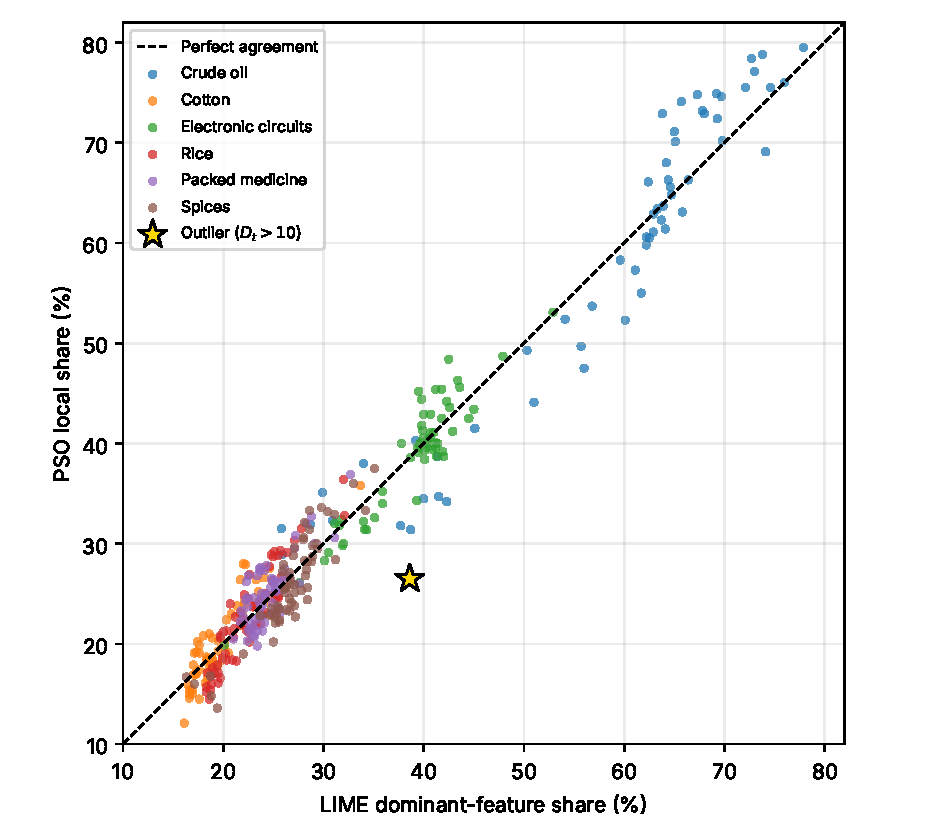
\includegraphics[width=0.88\linewidth]{figures/lime_pso_scatter.pdf}
\caption{Scatter plot of LIME dominant-feature share versus PSO local share for all 360 sector-month observations, colour-coded by sector. The dashed diagonal marks perfect LIME--PSO agreement. Points lie close to the diagonal in all six sectors, with the widest spread for crude oil; the single outlying point (starred) is October~2025 for crude oil ($D_t=12.2$\,percentage points), the sole observation exceeding the 10-point threshold.}
\label{fig:lime_pso_scatter}
\end{figure}

\FloatBarrier

\section{Comparison with Related Studies}
The related-work section cites a fair number of papers, and lining all of them up against ours would only give a long table that nobody reads. So we kept four, each standing for a different strand of that discussion: Balasubramanian and Natarajan \cite{balasubramanian2026} on Indian monthly trade, Chinn et al.\ \cite{chinn2023} on trade nowcasting, Canti et al.\ \cite{canti2024} on temporal explanations, and Gao et al.\ \cite{gao2024} on PSO-based feature selection. A caveat comes first. These studies use different data and report different error measures, so a side-by-side accuracy table would say very little. What can be compared fairly is the scope of each study, meaning what it actually sets out to do. We therefore asked six questions of every paper: whether it works on trade data, whether it uses Indian monthly series, whether it uses PSO to optimise the features, whether it explains individual months locally, whether it tracks attribution across time, and whether it links event labels to an explanation-agreement check. Figure~\ref{fig:related} shows the answers. A filled circle means the study clearly does this according to its published abstract, and an empty one means it does not or that we could not confirm it.

\begin{figure}[!ht]
\centering
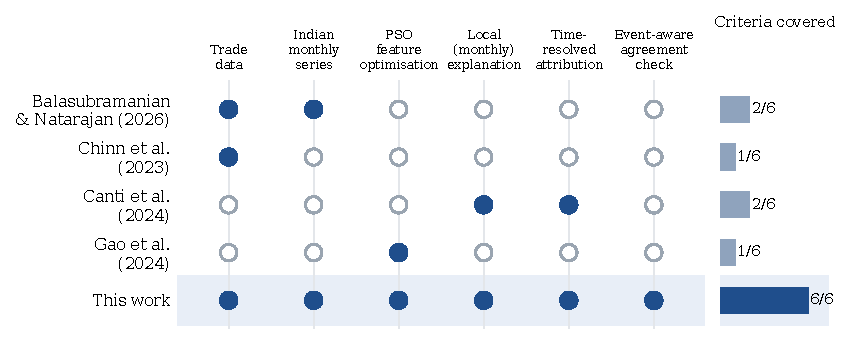
\includegraphics[width=\textwidth]{figures/related_work_comparison.pdf}
\caption{Scope comparison of four studies from the related-work section against the present framework. Filled circles mark the criteria that a study addresses according to its published abstract; the bars on the right count the criteria covered out of six. The comparison concerns scope, not forecasting accuracy.}
\label{fig:related}
\end{figure}

Balasubramanian and Natarajan are closest to us in terms of data. They also work with monthly Indian trade and make feature importance their main result, but they use aggregate export and import values from 1990--91 to 2024--25 with tree-based models, so what comes out is one importance picture for the whole period. It cannot tell you why a particular month looks unusual. Chinn et al.\ are after something else: their three-step approach (pre-selection, factor extraction, then a machine-learning regression) is aimed at forecasting world trade across several horizons, and explaining individual predictions is not part of the design. Canti et al.\ are almost the mirror image. They compare SHAP, LIME and Integrated Gradients on time-series predictions and ask which moments drive a result, yet their data is not trade data and there is neither an optimiser nor any event labelling in the picture. Gao et al.\ propose a PSO variant that ranks features by information gain ratio and decides, for each feature, whether to keep it. It was tested on 16 datasets. In our case PSO does not select anything; it assigns a continuous weight to every predictor, and that weight vector is what the monthly LIME shares are later compared with.

Put next to each other, no single one of the four covers more than two of the six questions, whereas the framework in this paper covers all six. This should not be read as a claim that our model forecasts better. We did not run the other methods on our data, and the figure says nothing about accuracy. What it does show is where the contribution sits: in combining event labels, PSO weights, monthly LIME, yearly SHAP and an agreement check inside one workflow for Indian commodities, which is how we described it earlier. One more limit applies. The scores come from our own reading of the abstracts, and a study may well do more than its abstract states.

\FloatBarrier

\clearpage
\section{Temporal XAI Interpretation}
Across all 360 monthly observations, the mean LIME--PSO difference is 2.16 percentage points and only one month exceeds the 10-point threshold. The sole outlier is October 2025 for crude oil, which is REGULAR under the event rule with $z=0.49$. Domestic consumption is the dominant LIME variable for this month, with a 38.6\% local share, while the PSO-induced local share for the same feature is 26.5\%, producing a 12.2-point difference. None of the 44 SURGE/DROP observations is an outlier, and the largest event-month difference remains below six percentage points. This separation between event status and explanation-outlier status is central to the interpretation. The z-score classifies the magnitude of a monthly target movement relative to the historical distribution of changes, while the LIME--PSO test assesses whether the local explanatory distribution remains broadly consistent with the globally optimised feature-weight structure. A high event magnitude therefore does not imply a high explanation disagreement, and a regular month can still become a diagnostic outlier. The event-classification layer and the LIME–PSO comparison layer provide complementary information and cannot replace each other because they answer different questions.

The yearly SHAP profiles show persistent but commodity-specific attribution structures. Crude oil trade was mostly influenced by domestic consumption across all five years, with stock change, investment, and exchange-rate variables also appearing among the leading contributors. Cotton trade was dominated by stock change, domestic production, and domestic wholesale prices. Electronic circuits retains domestic consumption as its leading annual contributor while export-value and export-quantity variables remain prominent. Rice is repeatedly characterised by stock change and production, while the global benchmark price becomes comparatively more important in 2025. Packed medicine places substantial annual attribution on opening stock, closing stock, and production, whereas spices repeatedly place production and stock change among the largest yearly contributors. These profiles show why a single static feature ranking is inadequate for a monthly trade framework: the factor that dominates one month can differ from the variable that dominates an annual average. Recent temporal-XAI research similarly emphasises preserving when a feature matters rather than reducing the sequence to one global ranking \cite{canti2024,vanzy2024,hertel2026}. The yearly SHAP layer therefore acts as a temporal complement to the monthwise LIME analysis.

PSO, LIME, and SHAP explain different perspectives while working on the same data. PSO provides a global weight vector with weights assigned to each feature. LIME examines which feature contributes the most to the prediction for a particular month, whereas SHAP provides an aggregate, sector-specific annual summary of feature contributions. The common 0--100\% scale allows LIME and PSO to be compared. The mean difference of 2.16 percentage points and the fact that 359 of 360 observations lie at or below the 10-point threshold indicate broad agreement under this selected diagnostic scale. The crude oil outlier illustrates why the comparison is useful: the model's monthly explanation differs significantly from the global weighting vector, even though the month is classified as REGULAR. The trade dataset contains variables that are connected, either through their economic relationships or through the way certain values are calculated, because of which LIME and SHAP explanations alone cannot establish which factors actually caused a change in trade but can only explain how the model uses these variables to make predictions. This framework provides an approach to analysing fluctuations in Indian trade. The five-year sample provides a data-based application of the framework.

Table~\ref{tab:shap} and Fig.~\ref{fig:shap} together show how the leading attribution changes by sector and year. The ranking is necessary for examining patterns in feature contributions. The consistent dominance of the same feature across several years suggests that the model gives more importance to that feature. However, changes in the ranking of the dominant feature from one year to another do not necessarily indicate changes in the underlying causes of trade, but rather shifts in the model's attribution. The heatmap provides a visual representation that makes it easier to compare changes in attribution patterns over the five-year period.

\begin{figure}[!ht]
\centering
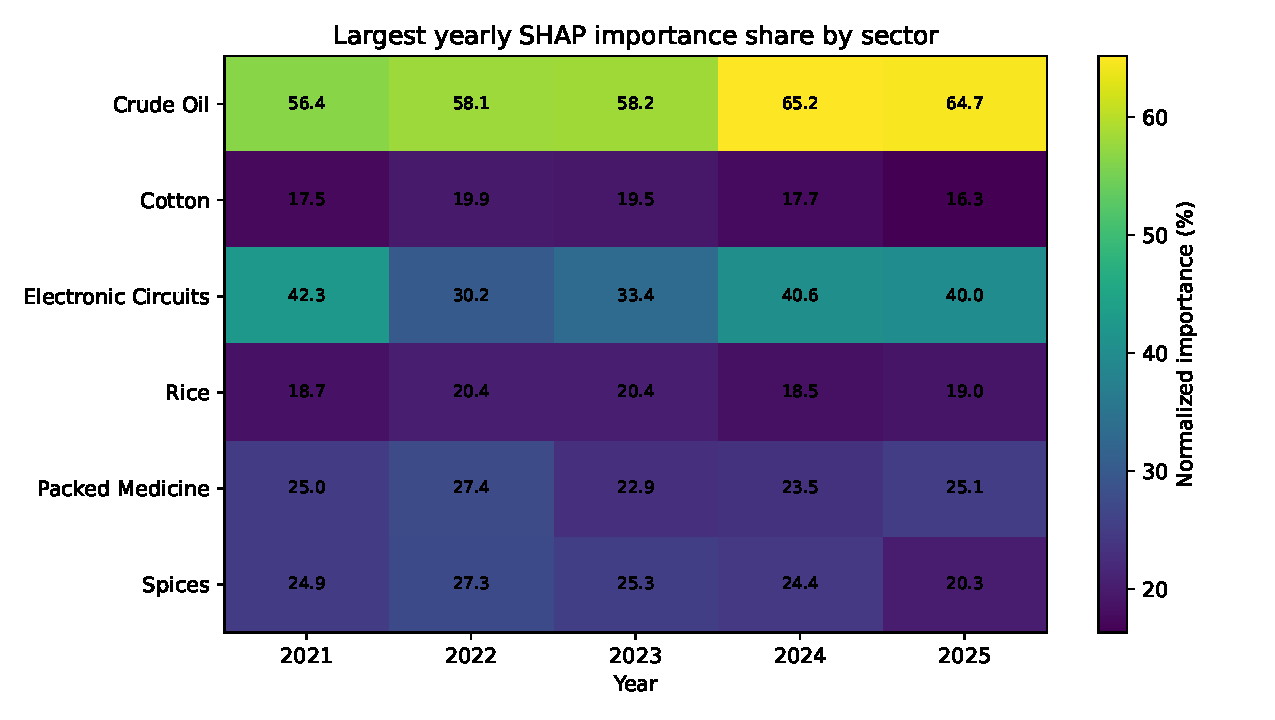
\includegraphics[width=0.96\linewidth]{figures/shap_yearly_heatmap.pdf}
\caption{Yearly SHAP importance profiles. Values are normalised absolute contribution shares within each sector-year.}
\label{fig:shap}
\end{figure}

\FloatBarrier\nobreak\vspace{4pt}\nobreak

\captionsetup[table]{position=below}
\begin{table}[ht]
\centering
\setlength{\tabcolsep}{4pt}
\tiny
\renewcommand{\arraystretch}{1.45}
\small
\begin{tabular}{%
  >{\raggedright\arraybackslash}p{2.0cm}%  Sector
  >{\raggedright\arraybackslash}p{1.85cm}%  2021
  >{\raggedright\arraybackslash}p{1.85cm}%  2022
  >{\raggedright\arraybackslash}p{1.85cm}%  2023
  >{\raggedright\arraybackslash}p{1.85cm}%  2024
  >{\raggedright\arraybackslash}p{1.85cm}%  2025
}
\toprule
\textbf{Sector} & \textbf{2021} & \textbf{2022} & \textbf{2023} & \textbf{2024} & \textbf{2025}\\
\midrule
\addlinespace[3pt]
Crude oil
  & Cons\ \ 56.4\newline dStk\ \ 13.7\newline Capex 10.7
  & Cons\ \ 58.1\newline dStk\ \ 16.7\newline FX\ \ \ \ \ 7.1
  & Cons\ \ 58.2\newline dStk\ \ 16.8\newline FX\ \ \ \ \ 9.2
  & Cons\ \ 65.2\newline Capex 10.0\newline dStk\ \ \ 9.9
  & Cons\ \ 64.7\newline Capex 10.8\newline dStk\ \ 10.6\\
\addlinespace[4pt]
Cotton
  & dStk\ \ 17.5\newline Prod\ \ 17.3\newline Capex 15.9
  & dStk\ \ 19.9\newline Prod\ \ 19.6\newline WPI\ \ 18.4
  & Prod\ \ 19.5\newline dStk\ \ 19.2\newline WPI\ \ 13.7
  & WPI\ \ 17.7\newline Prod\ \ 15.1\newline dStk\ \ 14.5
  & WPI\ \ 16.3\newline Capex 16.2\newline dStk\ \ 15.3\\
\addlinespace[4pt]
Electronic\newline circuits
  & Cons\ \ 42.3\newline ExpV\ 19.0\newline ExpQ 13.8
  & Cons\ \ 30.2\newline ExpV\ 21.7\newline ExpQ 15.2
  & Cons\ \ 33.4\newline ExpV\ 20.4\newline ExpQ 15.2
  & Cons\ \ 40.6\newline ExpV\ 18.2\newline ExpQ 13.5
  & Cons\ \ 40.0\newline ExpV\ 18.9\newline ExpQ 13.4\\
\addlinespace[4pt]
Rice
  & dStk\ \ 18.7\newline Prod\ \ 18.5\newline GPr\ \ 16.7
  & dStk\ \ 20.4\newline Prod\ \ 20.2\newline ImpQ\ 18.4
  & Prod\ \ 20.4\newline dStk\ \ 20.3\newline ImpQ\ 19.9
  & Prod\ \ 18.5\newline dStk\ \ 18.2\newline GPr\ \ 16.6
  & GPr\ \ 19.0\newline dStk\ \ 16.0\newline Prod\ \ 15.9\\
\addlinespace[4pt]
Packed\newline medicine
  & Prod\ \ 25.0\newline OStk\ 19.6\newline CStk\ 18.7
  & OStk\ 27.4\newline CStk\ 23.8\newline Prod\ \ 16.0
  & OStk\ 22.9\newline CStk\ 20.0\newline Prod\ \ 20.0
  & OStk\ 23.5\newline Prod\ \ 21.6\newline CStk\ 20.9
  & Prod\ \ 25.1\newline OStk\ 22.1\newline CStk\ 19.5\\
\addlinespace[4pt]
Spices
  & Prod\ \ 24.9\newline dStk\ \ 23.4\newline ImpQ\ 11.0
  & Prod\ \ 27.3\newline dStk\ \ 26.9\newline ImpQ\ \ 9.3
  & Prod\ \ 25.3\newline dStk\ \ 24.6\newline ImpQ\ 11.0
  & dStk\ \ 24.4\newline Prod\ \ 22.5\newline ImpQ\ \ 8.7
  & dStk\ \ 20.3\newline Prod\ \ 19.3\newline OStk\ 11.2\\
\addlinespace[3pt]
\bottomrule
\end{tabular}
\caption{Top three yearly SHAP features by sector, ranked by normalised importance share within
each sector-year. Each cell lists the top three features with their normalised absolute SHAP
contribution share (\%). Feature abbreviations: Cons = Domestic Consumption; Prod = Domestic
Production; dStk = Stock Change; OStk = Opening Stock; CStk = Closing Stock; WPI = Domestic
Wholesale Price; GPr = Global Benchmark Price; FX = Exchange Rate; Capex = Sector Investment;
ImpQ = Import Quantity; ExpV = Export Value; ExpQ = Export Quantity. Crude oil is consistently
led by domestic consumption (56--65\%); electronic circuits by domestic consumption (30--42\%);
and cotton, rice, packed medicine, and spices by production and stock-related variables
throughout 2021--2025.}
\label{tab:shap}
\end{table}
\captionsetup[table]{position=above}

\clearpage
\section{Discussion}

The results demonstrate that PSO, LIME, and SHAP provide complementary and broadly consistent explanations within the same feature space across all six Indian trade sectors. PSO searches for a globally optimised feature-weight vector over the 48-month calibration history; LIME constructs a local linear surrogate for each individual month; and SHAP decomposes the fitted response into additive annual contributions. Despite operating at different levels of temporal granularity, all three methods converge on the same dominant features in the vast majority of observations. On the common 0--100\,\% contribution-share scale, the cross-sector mean LIME--PSO difference is 2.16 percentage points across 360 observations, and 359 of 360 observations remain at or below the 10-point diagnostic threshold. None of the 44 SURGE or DROP event months registers as a LIME--PSO outlier, which indicates that heightened trade volatility does not systematically degrade the local-global explanation agreement. The outlier of October 2025 for crude oil, being classified as REGULAR ($z = 0.49$), explains that trade-event classification and disagreement in explanations are on different spectra. The SHAP explanations applied year-wise to each commodity show that each commodity has a specific pattern, which is mostly consistent across the five calendar years. For the crude oil sector, domestic demand makes a major contribution to the model's predictions across the five calendar years. It has a contribution of (56--65\%) in the SHAP results as India has world's third largest oil consumption. It suggests that domestic demand is associated with import quantity even when short-term price or policy conditions fluctuate. India's growing electronics manufacturing and assembly sector can be interpreted in light of the fact that domestic consumption was the consistent yearly leader, having (30--42\%) of the SHAP contribution. Cotton, rice, packed medicine, and spices are mostly influenced by stock changes and production factors because there are agricultural and seasonal constraints associated with these commodities. The major monthly LIME contributor differs from the major yearly SHAP contributor, which is why a single fixed ranking is not appropriate for analysing monthly trade patterns. This finding is consistent with recent research on temporal XAI, which highlights the importance of considering changes in feature contributions over time rather than relying on a single global importance ranking. \cite{canti2024,vanzy2024,hertel2026}.


The limitations of this framework include a short period of 60 months for analysis, which reduces the depth of the historical data available for calibration and makes it difficult to detect structural breaks reliably.  The 10-percentage-point diagnostic cutoff was selected based on a preliminary pilot analysis to understand how different threshold values affect the number of outliers. The response surface in the PSO stage is designed to remain simple and transparent, making it easier to examine the complete feature-weight vector and compare it with LIME explanations. Its main purpose is to support this comparison rather than to act as a general-purpose prediction model. Several input features are economically or mechanically related — for example, opening stock and closing stock — so attribution shares should not be interpreted as causal effects. The 1.5 z-score event threshold is fixed across all sectors; an adaptive or sector-specific threshold could shift the event calendar and alter the count of SURGE and DROP observations. Finally, the LIME perturbation variance and ridge regularisation parameter are held constant across all 360 explanations; sensitivity to these settings has not been examined in this study.

\section{Conclusion}

This paper presents an integrated and reproducible Indian trade-analysis framework that connects monthly event detection, PSO-based global feature weighting, LIME local explanation, and SHAP temporal attribution in a single pipeline applied to six commodity sectors over January 2021 to December 2025. The framework maps crude oil, cotton, and electronic circuits to international-demand tasks and rice, packed medicine, and spices to international-supply tasks, yielding 360 sector-month observations in total. Using the 1.5 threshold for z-score event classification, 26 months are classified as SURGE, 18 as DROP, and the remaining 316 as REGULAR. The global best ($gbest$) vector, which assigns weights to each factor, is obtained by PSO for each sector within 250 iterations. The local monthly contributions are obtained from LIME. SHAP is used to summarise feature contributions for each year. The mean LIME–PSO difference obtained on the 0–100\% standardised scale was 2.16 percentage points, and there was only one outlier out of 360 observations, which gives an outlier rate of 0.28\%. Therefore, the two methods generally show a high level of agreement in their explanations. The yearly SHAP heatmap helps to visualise commodity-specific patterns, which are mostly consistent over time, and further explains the LIME results. The complete computational package, including fixed random seeds, sector-specific PSO implementations, and all output tables, is designed for full reproducibility. Future research on this topic should expand the dataset to more than 60 months and include more sectors and macroeconomic variables. It can include expanding calibration windows and then examine whether low LIME–PSO comparison scores are observed in alternative models.The direction of Indian trade can be better understood if explanation outliers are identified in advance so that the months that require further investigation can be flagged.
\section{Declaration}
\textbf{Author Contributions:}\\\\
T.K.M. conceptualized the research problem and supervised the study. A.P. designed
and implemented the proposed framework, conducted the experiments, analyzed the
results, and prepared the manuscript. All authors reviewed and approved the final
manuscript.\\\\
\textbf{Conflict of Interest}\\
The authors declare that they have no conflict of interest.\\\\
\textbf{Funding Information}\\
No funding was received for this research work.\\\\
\textbf{Ethical Consideration} Not Applicable.\\
\textbf{Data \& Code Availability}\\
The underlying monthly commodity-level import and export data used in this study are publicly available through the Government of India, Department of Commerce, TRADESTAT portal (\url{https://tradestat.commerce.gov.in/}). The processed dataset covering the six commodity sectors from January 2021 to December 2025, together with the source code, fixed random seeds, instructions, and files required to reproduce the reported results, tables, and figures, is publicly available at \url{https://github.com/aaradhypandey/indian-trade-xai}. No confidential or personally identifiable data were used in this study.
\clearpage
\begin{thebibliography}{99}

% [1] Josic & Zmuk 2022 — GENUINE. Published in Business Systems Research (De Gruyter).
\bibitem{josic2022} H. Jo{\v{s}}i{\'c}, B. {\v{Z}}muk, A machine learning approach to forecast international trade: The case of Croatia. Bus. Syst. Res. \textbf{13}(3), 144--160 (2022). \url{https://doi.org/10.2478/bsrj-2022-0030}

% [2] Chinn, Meunier & Stumpner 2023 — NBER Working Paper 31419.
\bibitem{chinn2023} M.D. Chinn, B. Meunier, S. Stumpner, Nowcasting world trade with machine learning: A three-step approach. NBER Working Paper No. 31419 (2023). \url{https://doi.org/10.3386/w31419}

% [3] Yang, Lee & Chang 2023 — GENUINE. Published in Expert Systems with Applications (Elsevier).
\bibitem{yang2023} C.-H. Yang, C.-F. Lee, P.-Y. Chang, Export- and import-based economic models for predicting global trade using deep learning. Expert Syst. Appl. \textbf{218}, 119590 (2023). \url{https://doi.org/10.1016/j.eswa.2023.119590}

% [5] Guidotti et al. 2018 — GENUINE. ACM Computing Surveys, highly cited XAI survey.
\bibitem{guidotti2018} R. Guidotti, A. Monreale, S. Ruggieri, F. Turini, F. Giannotti, D. Pedreschi, A survey of methods for explaining black box models. ACM Comput. Surv. \textbf{51}(5), 93:1--93:42 (2018). \url{https://doi.org/10.1145/3236009}

% [6] Arrieta et al. 2020 — GENUINE. Information Fusion, leading XAI survey paper.
\bibitem{arrieta2020} A.B. Arrieta, N. D{\'i}az-Rodr{\'i}guez, J. Del Ser, A. Bennetot, S. Tabik, A. Barbado, S. Garcia, S. Gil-Lopez, D. Molina, R. Benjamins, R. Chatila, F. Herrera, Explainable Artificial Intelligence (XAI): Concepts, taxonomies, opportunities and challenges toward responsible AI. Inf. Fusion \textbf{58}, 82--115 (2020). \url{https://doi.org/10.1016/j.inffus.2019.12.012}

% [7] Schwalbe & Finzel 2024 — GENUINE. Data Mining and Knowledge Discovery (Springer).
\bibitem{schwalbe2024} G. Schwalbe, B. Finzel, A comprehensive taxonomy for explainable artificial intelligence: A systematic survey of surveys on methods and concepts. Data Min. Knowl. Discov. \textbf{38}, 3043--3101 (2024). \url{https://doi.org/10.1007/s10618-022-00867-8}

% [8] Mersha et al. 2024 — GENUINE. Neurocomputing (Elsevier).
\bibitem{mersha2024} M. Mersha, K. Lam, J. Wood, A.K. AlShami, J. Kalita, Explainable artificial intelligence: A survey of needs, techniques, applications, and future direction. Neurocomputing \textbf{599}, 128111 (2024). \url{https://doi.org/10.1016/j.neucom.2024.128111}

% [9] Abusitta, Li & Fung 2024 — GENUINE. Expert Systems with Applications (Elsevier).
\bibitem{abusitta2024} A. Abusitta, M.Q. Li, B.C.M. Fung, Survey on explainable AI: Techniques, challenges and open issues. Expert Syst. Appl. \textbf{255}, 124710 (2024). \url{https://doi.org/10.1016/j.eswa.2024.124710}

% [10] Longo et al. 2024 — GENUINE. Information Fusion (Elsevier). XAI 2.0 manifesto.
\bibitem{longo2024} L. Longo, M. Brcic, F. Cabitza, J. Choi, R. Confalonieri, J. Del Ser, R. Guidotti, Y. Hayashi, F. Herrera, A. Holzinger, et al., Explainable Artificial Intelligence (XAI) 2.0: A manifesto of open challenges and interdisciplinary research directions. Inf. Fusion \textbf{106}, 102301 (2024). \url{https://doi.org/10.1016/j.inffus.2024.102301}

% [11] TRADESTAT — Official Government of India trade data portal. No DOI; URL citation.
\bibitem{tradestat} Government of India, Department of Commerce, TRADESTAT: System on Monthly Foreign Trade Statistics of India (2026). Available at: \url{https://tradestat.commerce.gov.in/ftspcc/import_commodity_xcountry_wise_monthly}. Accessed 10 September 2026.

% [12] Balasubramanian & Natarajan 2026 — GENUINE. Engineering, Technology and Applied Science Research (ETASR).
\bibitem{balasubramanian2026} S. Balasubramanian, M. Natarajan, Feature learning behavior in trade forecasting: Evidence from tree-based machine learning models. Eng. Technol. Appl. Sci. Res. \textbf{16}(2), 34097--34101 (2026). \url{https://doi.org/10.48084/etasr.17612}

% [14] Ribeiro, Singh & Guestrin 2016 — GENUINE. The original LIME paper, KDD 2016.
\bibitem{ribeiro2016} M.T. Ribeiro, S. Singh, C. Guestrin, ``Why should I trust you?'': Explaining the predictions of any classifier. In: Proc. 22nd ACM SIGKDD International Conference on Knowledge Discovery and Data Mining, pp. 1135--1144 (2016). \url{https://doi.org/10.1145/2939672.2939778}

% [15] Lundberg & Lee 2017 — GENUINE. The original SHAP paper, NeurIPS 2017. DOI via arXiv preprint.
\bibitem{lundberg2017} S.M. Lundberg, S.-I. Lee, A unified approach to interpreting model predictions. In: Advances in Neural Information Processing Systems \textbf{30} (2017). \url{https://doi.org/10.48550/arXiv.1705.07874}

% [16] Aas, Jullum & Loland 2021 — GENUINE. Artificial Intelligence (Elsevier).
\bibitem{aas2021} K. Aas, M. Jullum, A. L{\o}land, Explaining individual predictions when features are dependent: More accurate approximations to Shapley values. Artif. Intell. \textbf{298}, 103502 (2021). \url{https://doi.org/10.1016/j.artint.2021.103502}

% [17] Janzing, Minorics & Blobaum 2020 — GENUINE. AISTATS 2020 (PMLR). DOI via arXiv.
\bibitem{janzing2020} D. Janzing, L. Minorics, P. Bl{\"o}baum, Feature relevance quantification in explainable AI: A causal problem. In: Proc. 23rd International Conference on Artificial Intelligence and Statistics, PMLR \textbf{108}, 2907--2916 (2020). \url{https://doi.org/10.48550/arXiv.1910.13413}

% [18] Canti et al. 2024 — GENUINE. IEEE BigDataService 2024.
\bibitem{canti2024} E. Canti, E. Collini, L.A. Ipsaro Palesi, P. Nesi, Comparing techniques for temporal explainable artificial intelligence. In: 2024 IEEE 10th International Conference on Big Data Computing Service and Machine Learning Applications, pp. 87--91 (2024). \url{https://doi.org/10.1109/BigDataService62917.2024.00019}

% [19] van Zyl, Ye & Naidoo 2024 — GENUINE. Applied Energy (Elsevier).
\bibitem{vanzy2024} C. van Zyl, X. Ye, R. Naidoo, Harnessing eXplainable artificial intelligence for feature selection in time series energy forecasting: A comparative analysis of Grad-CAM and SHAP. Appl. Energy \textbf{353}, 122079 (2024). \url{https://doi.org/10.1016/j.apenergy.2023.122079}

% [22] Hertel et al. 2026 — Nature Communications (Springer Nature).
\bibitem{hertel2026} M. Hertel, S. P{\"u}tz, R. Mikut, V. Hagenmeyer, B. Sch{\"a}fer, Explainable time-series forecasting with sampling-free SHAP for Transformers. Nat. Commun. \textbf{17}, 4723 (2026). \url{https://doi.org/10.1038/s41467-026-73243-5}

% [23] Kennedy & Eberhart 1995 — GENUINE. The original PSO paper, ICNN 1995.
\bibitem{kennedy1995} J. Kennedy, R. Eberhart, Particle swarm optimization. In: Proc. ICNN'95 -- International Conference on Neural Networks, IEEE, pp. 1942--1948 (1995). \url{https://doi.org/10.1109/ICNN.1995.488968}

% [24] Shi & Eberhart 1998 — GENUINE. IEEE ICEC 1998. Inertia weight PSO.
\bibitem{shi1998} Y. Shi, R.C. Eberhart, A modified particle swarm optimizer. In: 1998 IEEE International Conference on Evolutionary Computation, pp. 69--73 (1998). \url{https://doi.org/10.1109/ICEC.1998.699146}

% [25] Clerc & Kennedy 2002 — GENUINE. IEEE Transactions on Evolutionary Computation.
\bibitem{clerc2002} M. Clerc, J. Kennedy, The particle swarm---explosion, stability, and convergence in a multidimensional complex space. IEEE Trans. Evol. Comput. \textbf{6}(1), 58--73 (2002). \url{https://doi.org/10.1109/4235.985692}

% [26] Poli, Kennedy & Blackwell 2007 — GENUINE. Swarm Intelligence (Springer).
\bibitem{poli2007} R. Poli, J. Kennedy, T. Blackwell, Particle swarm optimization. Swarm Intell. \textbf{1}, 33--57 (2007). \url{https://doi.org/10.1007/s11721-007-0002-0}

% [28] Gao et al. 2024 — GENUINE. Knowledge-Based Systems (Elsevier).
\bibitem{gao2024} J. Gao, Z. Wang, T. Jin, J. Cheng, Z. Lei, S. Gao, Information gain ratio-based subfeature grouping empowers particle swarm optimization for feature selection. Knowl.-Based Syst. \textbf{286}, 111380 (2024). \url{https://doi.org/10.1016/j.knosys.2024.111380}

% [29] Gupta & Gupta 2024 — GENUINE. Knowledge-Based Systems (Elsevier).
\bibitem{gupta2024} S. Gupta, S. Gupta, Fitness and historical success information-assisted binary particle swarm optimization for feature selection. Knowl.-Based Syst. \textbf{306}, 112699 (2024). \url{https://doi.org/10.1016/j.knosys.2024.112699}

% [30] Jin et al. 2024 — GENUINE. Expert Systems with Applications (Elsevier).
\bibitem{jin2024} X. Jin, B. Wei, L. Deng, S. Yang, J. Zheng, F. Wang, An adaptive pyramid PSO for high-dimensional feature selection. Expert Syst. Appl. \textbf{257}, 125084 (2024). \url{https://doi.org/10.1016/j.eswa.2024.125084}

% [33] PEPSO feature-selection paper. Author list verified against SciOpen and the publisher record.
\bibitem{pepspso2025} S. Deng, M. Xie, B. Wang, S. Zhang, S. Guan, M. Li, Particle swarm optimization algorithm for feature selection inspired by peak ecosystem dynamics. Comput. Mater. Contin. \textbf{82}(2), 2723--2751 (2025). \url{https://doi.org/10.32604/cmc.2024.057874}

% [34] Rudin 2019 — GENUINE. Nature Machine Intelligence (Springer Nature). Highly cited.
\bibitem{rudin2019} C. Rudin, Stop explaining black box machine learning models for high stakes decisions and use interpretable models instead. Nat. Mach. Intell. \textbf{1}, 206--215 (2019). \url{https://doi.org/10.1038/s42256-019-0048-x}

% [35] Lipton 2018 — GENUINE. Communications of the ACM.
\bibitem{lipton2018} Z.C. Lipton, The mythos of model interpretability. Commun. ACM \textbf{61}(10), 36--43 (2018). \url{https://doi.org/10.1145/3233231}

\end{thebibliography}

\end{document}
